\documentclass[ignorenonframetext,]{beamer}
\setbeamertemplate{caption}[numbered]
\setbeamertemplate{caption label separator}{: }
\setbeamercolor{caption name}{fg=normal text.fg}
\beamertemplatenavigationsymbolsempty
\usepackage{lmodern}
\usepackage{amssymb,amsmath}
\usepackage{ifxetex,ifluatex}
\usepackage{fixltx2e} % provides \textsubscript
\ifnum 0\ifxetex 1\fi\ifluatex 1\fi=0 % if pdftex
  \usepackage[T1]{fontenc}
  \usepackage[utf8]{inputenc}
\else % if luatex or xelatex
  \ifxetex
    \usepackage{mathspec}
  \else
    \usepackage{fontspec}
  \fi
  \defaultfontfeatures{Ligatures=TeX,Scale=MatchLowercase}
\fi
\usetheme[]{CambridgeUS}
\usecolortheme{beaver}
\usefonttheme{structurebold}
% use upquote if available, for straight quotes in verbatim environments
\IfFileExists{upquote.sty}{\usepackage{upquote}}{}
% use microtype if available
\IfFileExists{microtype.sty}{%
\usepackage{microtype}
\UseMicrotypeSet[protrusion]{basicmath} % disable protrusion for tt fonts
}{}
\newif\ifbibliography
\hypersetup{
            pdftitle={A4 - Choroplethen - maptools und choreplethr},
            pdfauthor={Jan-Philipp Kolb},
            pdfborder={0 0 0},
            breaklinks=true}
\urlstyle{same}  % don't use monospace font for urls
\usepackage{color}
\usepackage{fancyvrb}
\newcommand{\VerbBar}{|}
\newcommand{\VERB}{\Verb[commandchars=\\\{\}]}
\DefineVerbatimEnvironment{Highlighting}{Verbatim}{commandchars=\\\{\}}
% Add ',fontsize=\small' for more characters per line
\usepackage{framed}
\definecolor{shadecolor}{RGB}{248,248,248}
\newenvironment{Shaded}{\begin{snugshade}}{\end{snugshade}}
\newcommand{\KeywordTok}[1]{\textcolor[rgb]{0.13,0.29,0.53}{\textbf{#1}}}
\newcommand{\DataTypeTok}[1]{\textcolor[rgb]{0.13,0.29,0.53}{#1}}
\newcommand{\DecValTok}[1]{\textcolor[rgb]{0.00,0.00,0.81}{#1}}
\newcommand{\BaseNTok}[1]{\textcolor[rgb]{0.00,0.00,0.81}{#1}}
\newcommand{\FloatTok}[1]{\textcolor[rgb]{0.00,0.00,0.81}{#1}}
\newcommand{\ConstantTok}[1]{\textcolor[rgb]{0.00,0.00,0.00}{#1}}
\newcommand{\CharTok}[1]{\textcolor[rgb]{0.31,0.60,0.02}{#1}}
\newcommand{\SpecialCharTok}[1]{\textcolor[rgb]{0.00,0.00,0.00}{#1}}
\newcommand{\StringTok}[1]{\textcolor[rgb]{0.31,0.60,0.02}{#1}}
\newcommand{\VerbatimStringTok}[1]{\textcolor[rgb]{0.31,0.60,0.02}{#1}}
\newcommand{\SpecialStringTok}[1]{\textcolor[rgb]{0.31,0.60,0.02}{#1}}
\newcommand{\ImportTok}[1]{#1}
\newcommand{\CommentTok}[1]{\textcolor[rgb]{0.56,0.35,0.01}{\textit{#1}}}
\newcommand{\DocumentationTok}[1]{\textcolor[rgb]{0.56,0.35,0.01}{\textbf{\textit{#1}}}}
\newcommand{\AnnotationTok}[1]{\textcolor[rgb]{0.56,0.35,0.01}{\textbf{\textit{#1}}}}
\newcommand{\CommentVarTok}[1]{\textcolor[rgb]{0.56,0.35,0.01}{\textbf{\textit{#1}}}}
\newcommand{\OtherTok}[1]{\textcolor[rgb]{0.56,0.35,0.01}{#1}}
\newcommand{\FunctionTok}[1]{\textcolor[rgb]{0.00,0.00,0.00}{#1}}
\newcommand{\VariableTok}[1]{\textcolor[rgb]{0.00,0.00,0.00}{#1}}
\newcommand{\ControlFlowTok}[1]{\textcolor[rgb]{0.13,0.29,0.53}{\textbf{#1}}}
\newcommand{\OperatorTok}[1]{\textcolor[rgb]{0.81,0.36,0.00}{\textbf{#1}}}
\newcommand{\BuiltInTok}[1]{#1}
\newcommand{\ExtensionTok}[1]{#1}
\newcommand{\PreprocessorTok}[1]{\textcolor[rgb]{0.56,0.35,0.01}{\textit{#1}}}
\newcommand{\AttributeTok}[1]{\textcolor[rgb]{0.77,0.63,0.00}{#1}}
\newcommand{\RegionMarkerTok}[1]{#1}
\newcommand{\InformationTok}[1]{\textcolor[rgb]{0.56,0.35,0.01}{\textbf{\textit{#1}}}}
\newcommand{\WarningTok}[1]{\textcolor[rgb]{0.56,0.35,0.01}{\textbf{\textit{#1}}}}
\newcommand{\AlertTok}[1]{\textcolor[rgb]{0.94,0.16,0.16}{#1}}
\newcommand{\ErrorTok}[1]{\textcolor[rgb]{0.64,0.00,0.00}{\textbf{#1}}}
\newcommand{\NormalTok}[1]{#1}
\usepackage{longtable,booktabs}
\usepackage{caption}
% These lines are needed to make table captions work with longtable:
\makeatletter
\def\fnum@table{\tablename~\thetable}
\makeatother
\usepackage{graphicx,grffile}
\makeatletter
\def\maxwidth{\ifdim\Gin@nat@width>\linewidth\linewidth\else\Gin@nat@width\fi}
\def\maxheight{\ifdim\Gin@nat@height>\textheight0.8\textheight\else\Gin@nat@height\fi}
\makeatother
% Scale images if necessary, so that they will not overflow the page
% margins by default, and it is still possible to overwrite the defaults
% using explicit options in \includegraphics[width, height, ...]{}
\setkeys{Gin}{width=\maxwidth,height=\maxheight,keepaspectratio}

% Prevent slide breaks in the middle of a paragraph:
\widowpenalties 1 10000
\raggedbottom

\AtBeginPart{
  \let\insertpartnumber\relax
  \let\partname\relax
  \frame{\partpage}
}
\AtBeginSection{
  \ifbibliography
  \else
    \let\insertsectionnumber\relax
    \let\sectionname\relax
    \frame{\sectionpage}
  \fi
}
\AtBeginSubsection{
  \let\insertsubsectionnumber\relax
  \let\subsectionname\relax
  \frame{\subsectionpage}
}

\setlength{\parindent}{0pt}
\setlength{\parskip}{6pt plus 2pt minus 1pt}
\setlength{\emergencystretch}{3em}  % prevent overfull lines
\providecommand{\tightlist}{%
  \setlength{\itemsep}{0pt}\setlength{\parskip}{0pt}}
\setcounter{secnumdepth}{0}

\title{A4 - Choroplethen - \texttt{maptools} und \texttt{choreplethr}}
\author{Jan-Philipp Kolb}
\date{22 Oktober 2018}

\begin{document}
\frame{\titlepage}

\begin{frame}[fragile]{Inhalt dieses Abschnitts}

\begin{itemize}
\tightlist
\item
  Der Beispieldatensatz \texttt{wrld\_simpl} im Paket \texttt{maptools}
  wird vorgestellt.
\item
  Es wird gezeigt, wie man Daten aus anderen Quellen mit Kartendaten
  verbinden kann.
\item
  Mit dieser Verbindung ist es dann möglich thematische Karten - so
  genannte Choroplethen - zu erstellen
\item
  Zudem wird das Paket \texttt{choroplethr} vorgestellt.
\end{itemize}

\end{frame}

\begin{frame}{Was ist ein Choropleth}

Ein Choropleth ist eine Karte, die

\begin{itemize}
\tightlist
\item
  geografische Grenzen zeigt.
\item
  bei denen Bereiche basierend auf Metriken eingefärbt werden.
\end{itemize}

Choroplethen sind nützlich für die Visualisierung von Daten, wo
geografische Grenzen eine natürliche Einheit der Aggregation sind.

\end{frame}

\begin{frame}[fragile]{Das Paket \texttt{maptools}}

\begin{itemize}
\tightlist
\item
  Datensatz wrld\_simpl aus dem Paket \texttt{maptools}
\item
  Polygone für fast alle Staaten der Erde
\end{itemize}

\begin{Shaded}
\begin{Highlighting}[]
\KeywordTok{library}\NormalTok{(maptools)}
\KeywordTok{data}\NormalTok{(wrld_simpl)}
\end{Highlighting}
\end{Shaded}

\begin{longtable}[]{@{}lllrr@{}}
\toprule
& ISO2 & NAME & AREA & POP2005\tabularnewline
\midrule
\endhead
ATG & AG & Antigua and Barbuda & 44 & 83039\tabularnewline
DZA & DZ & Algeria & 238174 & 32854159\tabularnewline
AZE & AZ & Azerbaijan & 8260 & 8352021\tabularnewline
ALB & AL & Albania & 2740 & 3153731\tabularnewline
ARM & AM & Armenia & 2820 & 3017661\tabularnewline
AGO & AO & Angola & 124670 & 16095214\tabularnewline
\bottomrule
\end{longtable}

\end{frame}

\begin{frame}[fragile]{Hallo Welt}

\begin{Shaded}
\begin{Highlighting}[]
\KeywordTok{plot}\NormalTok{(wrld_simpl)}
\end{Highlighting}
\end{Shaded}

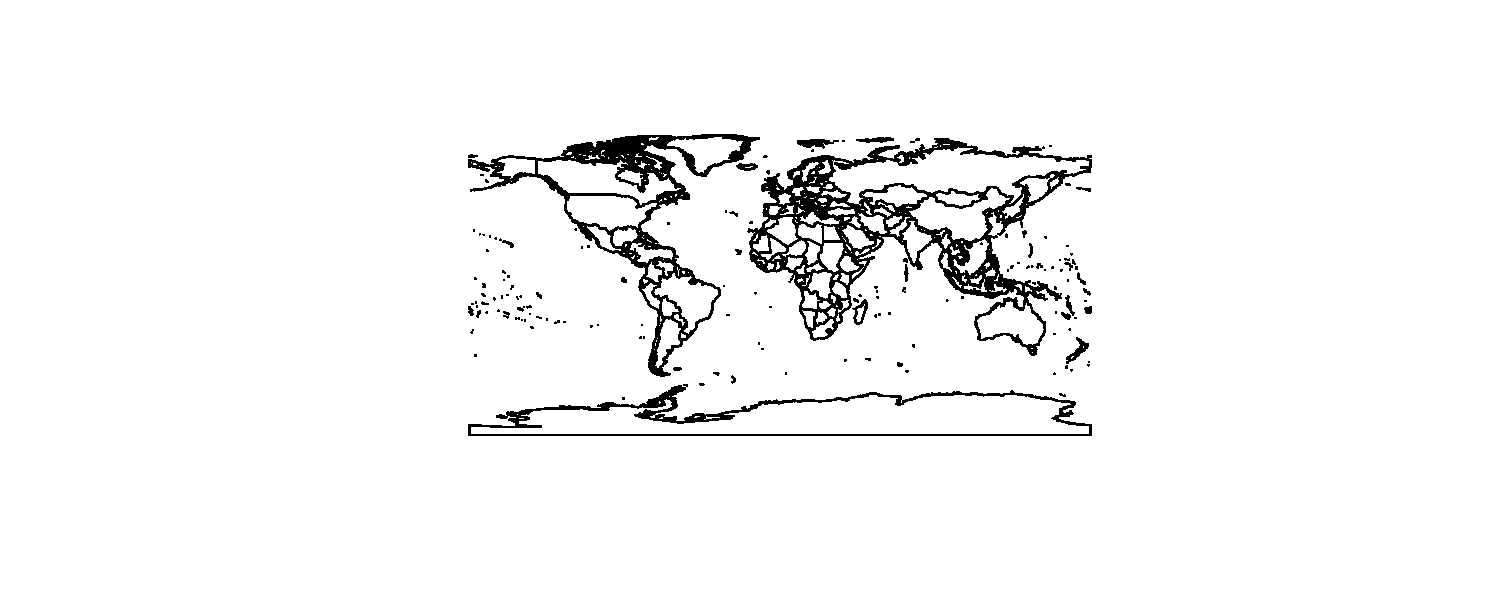
\includegraphics{Choroplethen_files/figure-beamer/unnamed-chunk-4-1.pdf}

\end{frame}

\begin{frame}[fragile]{\href{https://datahub.io/core/gini-index\#data}{Daten
zum Gini Index}}

\begin{itemize}
\tightlist
\item
  Daten von
  \href{https://datahub.io/core/gini-index\#data}{\textbf{datahub.io}}
\item
  Statistisches Maß zur Darstellung von
  \href{https://de.wikipedia.org/wiki/Gini-Koeffizient}{Ungleichverteilungen}
\end{itemize}

\begin{Shaded}
\begin{Highlighting}[]
\NormalTok{gini <-}\StringTok{ }\KeywordTok{read.csv}\NormalTok{(}\StringTok{"../data/gini-index_csv.csv"}\NormalTok{)}
\end{Highlighting}
\end{Shaded}

\begin{longtable}[]{@{}llrr@{}}
\toprule
Country.Name & Country.Code & Year & Value\tabularnewline
\midrule
\endhead
Albania & ALB & 1996 & 27.0\tabularnewline
Albania & ALB & 2002 & 31.7\tabularnewline
Albania & ALB & 2005 & 30.6\tabularnewline
Albania & ALB & 2008 & 30.0\tabularnewline
Albania & ALB & 2012 & 29.0\tabularnewline
Algeria & DZA & 1988 & 40.2\tabularnewline
\bottomrule
\end{longtable}

\end{frame}

\begin{frame}[fragile]{Der Gini Index im Jahr 2012}

\begin{itemize}
\tightlist
\item
  Für das Jahr 2012 sind am meisten Beobachtungen vorhanden.
\end{itemize}

\begin{Shaded}
\begin{Highlighting}[]
\NormalTok{gini12 <-}\StringTok{ }\NormalTok{gini[gini}\OperatorTok{$}\NormalTok{Year}\OperatorTok{==}\DecValTok{2012}\NormalTok{,]}
\KeywordTok{summary}\NormalTok{(gini12}\OperatorTok{$}\NormalTok{Value)}
\end{Highlighting}
\end{Shaded}

\begin{verbatim}
##    Min. 1st Qu.  Median    Mean 3rd Qu.    Max. 
##   24.70   29.80   35.10   36.15   41.40   57.40
\end{verbatim}

\end{frame}

\begin{frame}[fragile]{Exkurs: der Befehl \texttt{match}}

\begin{Shaded}
\begin{Highlighting}[]
\NormalTok{vec_a <-}\StringTok{ }\KeywordTok{c}\NormalTok{(}\StringTok{"A"}\NormalTok{,}\DecValTok{2}\NormalTok{,}\DecValTok{6}\NormalTok{,}\DecValTok{1}\NormalTok{,}\StringTok{"C"}\NormalTok{)}
\NormalTok{vec_b <-}\StringTok{ }\KeywordTok{c}\NormalTok{(}\DecValTok{1}\NormalTok{,}\StringTok{"C"}\NormalTok{,}\DecValTok{2}\NormalTok{)}

\KeywordTok{match}\NormalTok{(vec_a,vec_b)}
\end{Highlighting}
\end{Shaded}

\begin{verbatim}
## [1] NA  3 NA  1  2
\end{verbatim}

\end{frame}

\begin{frame}[fragile]{Die Daten matchen}

\begin{itemize}
\tightlist
\item
  WIr matchen die Gini-Daten mit den Kartendaten
\end{itemize}

\begin{Shaded}
\begin{Highlighting}[]
\NormalTok{ind <-}\StringTok{ }\KeywordTok{match}\NormalTok{(gini12}\OperatorTok{$}\NormalTok{Country.Code,wrld_simpl}\OperatorTok{$}\NormalTok{ISO3)}
\end{Highlighting}
\end{Shaded}

\begin{itemize}
\tightlist
\item
  Wir nehmen die Länder raus, für die keine Daten vorhanden sind:
\end{itemize}

\begin{Shaded}
\begin{Highlighting}[]
\NormalTok{ind2 <-}\StringTok{ }\NormalTok{ind[}\OperatorTok{!}\KeywordTok{is.na}\NormalTok{(ind)]}
\end{Highlighting}
\end{Shaded}

\begin{itemize}
\tightlist
\item
  Eine neue Karte wird erstellt:
\end{itemize}

\begin{Shaded}
\begin{Highlighting}[]
\NormalTok{ginimap <-}\StringTok{ }\NormalTok{wrld_simpl[ind2,]}
\end{Highlighting}
\end{Shaded}

\begin{itemize}
\tightlist
\item
  Die Gini-Daten werden in den Datenslot geschrieben
\end{itemize}

\begin{Shaded}
\begin{Highlighting}[]
\NormalTok{ginimap}\OperatorTok{@}\NormalTok{data}\OperatorTok{$}\NormalTok{gini12 <-}\StringTok{ }\NormalTok{gini12}\OperatorTok{$}\NormalTok{Value[}\OperatorTok{!}\KeywordTok{is.na}\NormalTok{(ind)]}
\end{Highlighting}
\end{Shaded}

\end{frame}

\begin{frame}[fragile]{Die Daten plotten}

\begin{Shaded}
\begin{Highlighting}[]
\KeywordTok{library}\NormalTok{(sp)}
\KeywordTok{spplot}\NormalTok{(ginimap,}\StringTok{"gini12"}\NormalTok{)}
\end{Highlighting}
\end{Shaded}

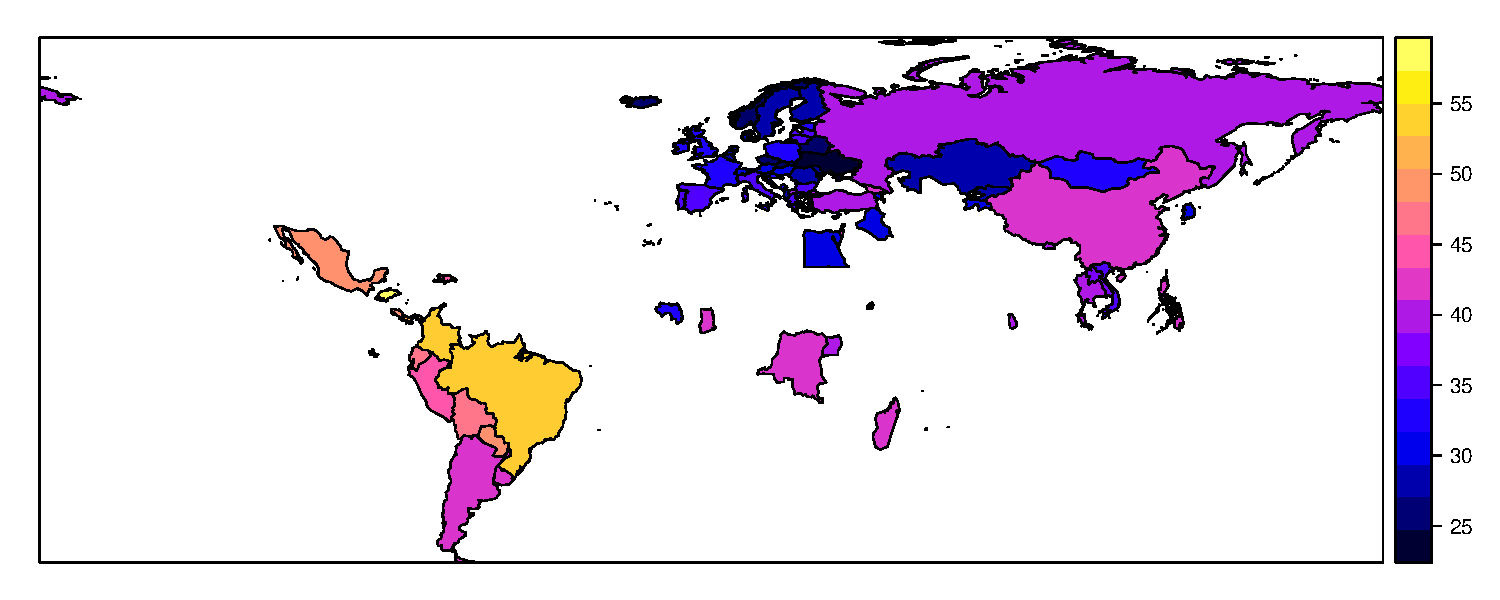
\includegraphics{Choroplethen_files/figure-beamer/unnamed-chunk-13-1.pdf}

\end{frame}

\begin{frame}[fragile]{Aufgabe A4A - Eine Choroplethenkarte erzeugen}

\begin{itemize}
\tightlist
\item
  Lade Datensatz
  \href{https://raw.githubusercontent.com/Japhilko/GeoData/master/2015/data/Unemployment.csv}{\textbf{Unemployment
  Datensatz}} herunter
\item
  Matche die Daten mit einer passenden Karte
\item
  Erzeuge mit der (Variable \texttt{X2014M10}) folgende Karte:
\end{itemize}

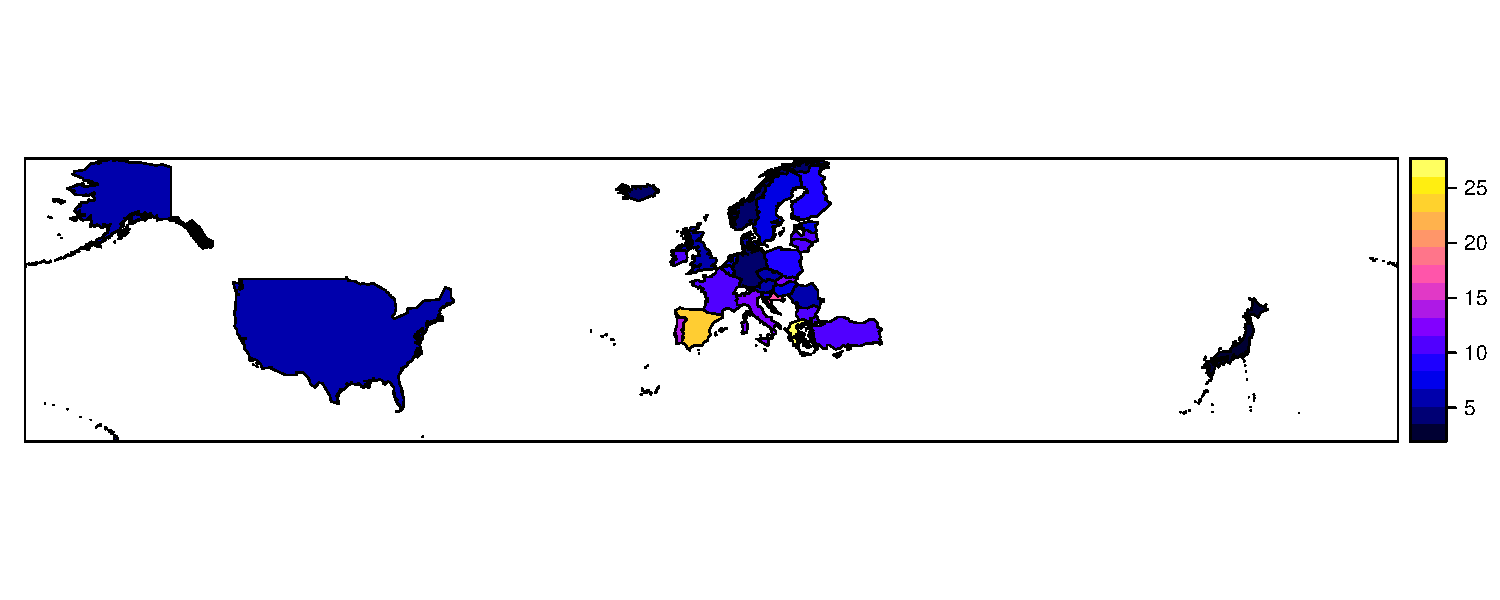
\includegraphics{Choroplethen_files/figure-beamer/unnamed-chunk-14-1.pdf}

\end{frame}

\begin{frame}[fragile]{Das Paket \texttt{choroplethr}}

\begin{block}{Paket von \href{http://www.arilamstein.com/}{\textbf{Ari
Lamstein}} -
\href{https://cran.r-project.org/web/packages/choroplethr/index.html}{\textbf{\texttt{choroplethr}}}}

\begin{itemize}
\item
  Vereinfachung der Erstellung von Choroplethen in R
\item
  World Development Indicators
  \href{https://cran.r-project.org/web/packages/WDI/index.html}{\textbf{\texttt{WDI}}}
  (World Bank)
\item
  Die folgenden Beispiele basieren auf der
  \href{https://cran.r-project.org/web/packages/choroplethr/index.html}{\textbf{Vignette}}
  des \texttt{choroplethr}-Paketes
\end{itemize}

\begin{Shaded}
\begin{Highlighting}[]
\KeywordTok{install.packages}\NormalTok{(}\StringTok{"choroplethr"}\NormalTok{)}
\end{Highlighting}
\end{Shaded}

\end{block}

\end{frame}

\begin{frame}[fragile]{Bevölkerungsschätzungen für den US-Staaten}

\texttt{df\_pop\_state} ist ein Datensatz , der in dem Paket
\texttt{choroplethr} enthalten ist, es enthält Schätzungen zu den
US-Staaten für das Jahr 2012.

\begin{longtable}[]{@{}lr@{}}
\toprule
region & value\tabularnewline
\midrule
\endhead
alabama & 4777326\tabularnewline
alaska & 711139\tabularnewline
arizona & 6410979\tabularnewline
arkansas & 2916372\tabularnewline
california & 37325068\tabularnewline
colorado & 5042853\tabularnewline
\bottomrule
\end{longtable}

\end{frame}

\begin{frame}[fragile]{\texttt{choroplethr} -
\href{http://mirrors.softliste.de/cran/web/packages/choroplethr/vignettes/a-introduction.html}{Hallo
Welt}}

Die Karte zeigt die US Bevölkerungsschätzung für die US-Staaten und das
Jahr 2012:

Wir bekommen eine Choroplethenkarte mit nur einem Argument:

\begin{Shaded}
\begin{Highlighting}[]
\KeywordTok{state_choropleth}\NormalTok{(df_pop_state)}
\end{Highlighting}
\end{Shaded}


\includegraphics{Choroplethen_files/figure-beamer/unnamed-chunk-20-1.pdf}

Aber wir können auch einen Titel erstellen und die Legende benennen:

\begin{Shaded}
\begin{Highlighting}[]
\KeywordTok{state_choropleth}\NormalTok{(df_pop_state, }\DataTypeTok{title=}\StringTok{"2012 US State Population Estimates"}\NormalTok{, }\DataTypeTok{legend=}\StringTok{"Population"}\NormalTok{)}
\end{Highlighting}
\end{Shaded}

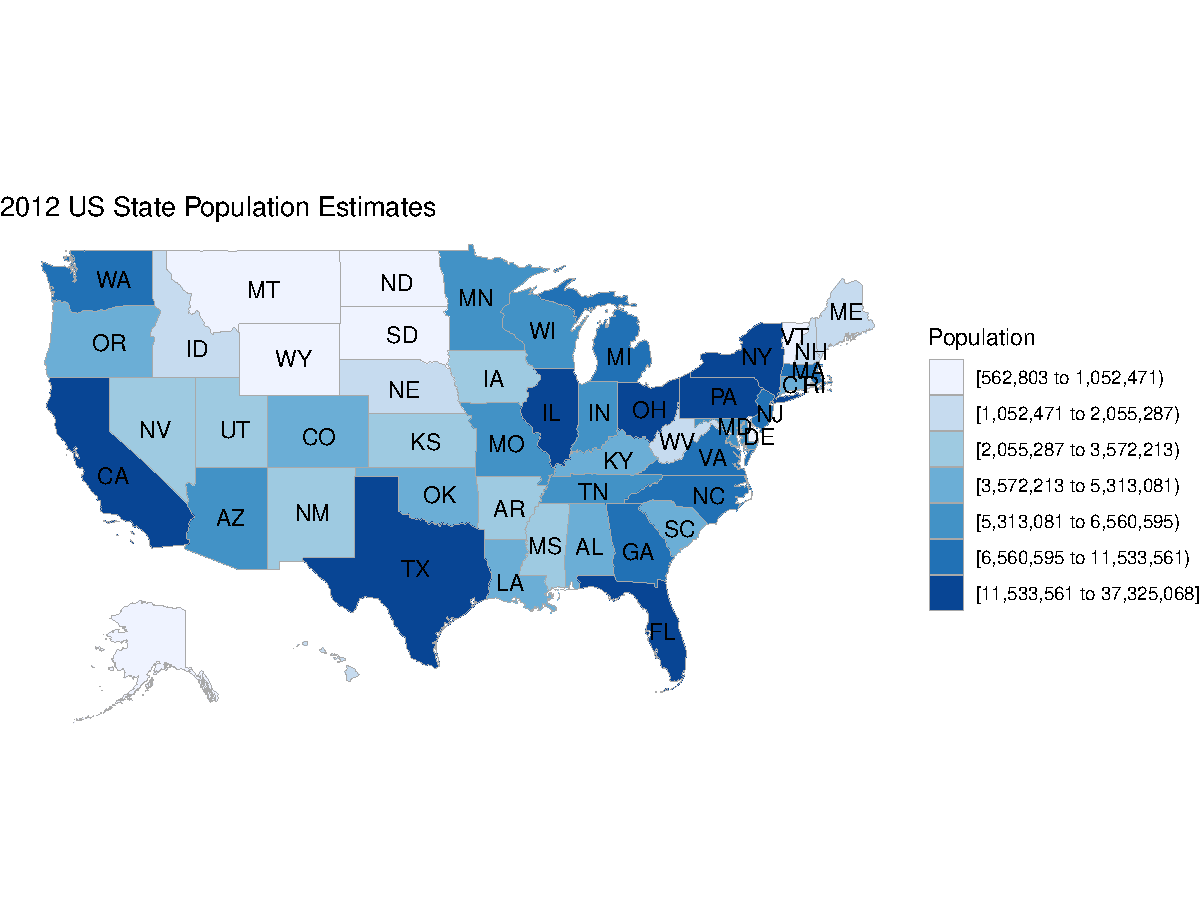
\includegraphics{Choroplethen_files/figure-beamer/unnamed-chunk-21-1.pdf}

\end{frame}

\begin{frame}[fragile]{\href{http://mirrors.softliste.de/cran/web/packages/choroplethr/vignettes/b-state-choropleth.html}{Nur
drei Staaten darstellen}}

\begin{Shaded}
\begin{Highlighting}[]
\KeywordTok{state_choropleth}\NormalTok{(df_pop_state,}
                 \DataTypeTok{title=} \StringTok{"2012 Population Estimates"}\NormalTok{,}
                 \DataTypeTok{legend=} \StringTok{"Population"}\NormalTok{, }\DataTypeTok{num_colors =} \DecValTok{1}\NormalTok{,}
                 \DataTypeTok{zoom=}\KeywordTok{c}\NormalTok{(}\StringTok{"california"}\NormalTok{,}\StringTok{"washington"}\NormalTok{,}\StringTok{"oregon"}\NormalTok{))}
\end{Highlighting}
\end{Shaded}


\includegraphics{Choroplethen_files/figure-beamer/unnamed-chunk-22-1.pdf}

\end{frame}

\begin{frame}[fragile]{US County Chroplethen}

\begin{block}{\href{http://mirrors.softliste.de/cran/web/packages/choroplethr/vignettes/c-county-choropleth.html}{Choroplethen
der US Counties}}

\begin{itemize}
\tightlist
\item
  \href{http://mirrors.softliste.de/cran/web/packages/choroplethr/vignettes/c-county-choropleth.html}{\textbf{Vignette
  des Pakets}}
\end{itemize}

\begin{Shaded}
\begin{Highlighting}[]
\CommentTok{# A data.frame containing population estimates for US Counties in 2012.}
\NormalTok{?df_pop_county}

\CommentTok{# Create a choropleth of US Counties}
\NormalTok{?county_choropleth}
\end{Highlighting}
\end{Shaded}

\end{block}

\end{frame}

\begin{frame}[fragile]{Eine Karte der US Counties}

\begin{Shaded}
\begin{Highlighting}[]
\KeywordTok{data}\NormalTok{(df_pop_county)}
\KeywordTok{county_choropleth}\NormalTok{(df_pop_county)}
\end{Highlighting}
\end{Shaded}

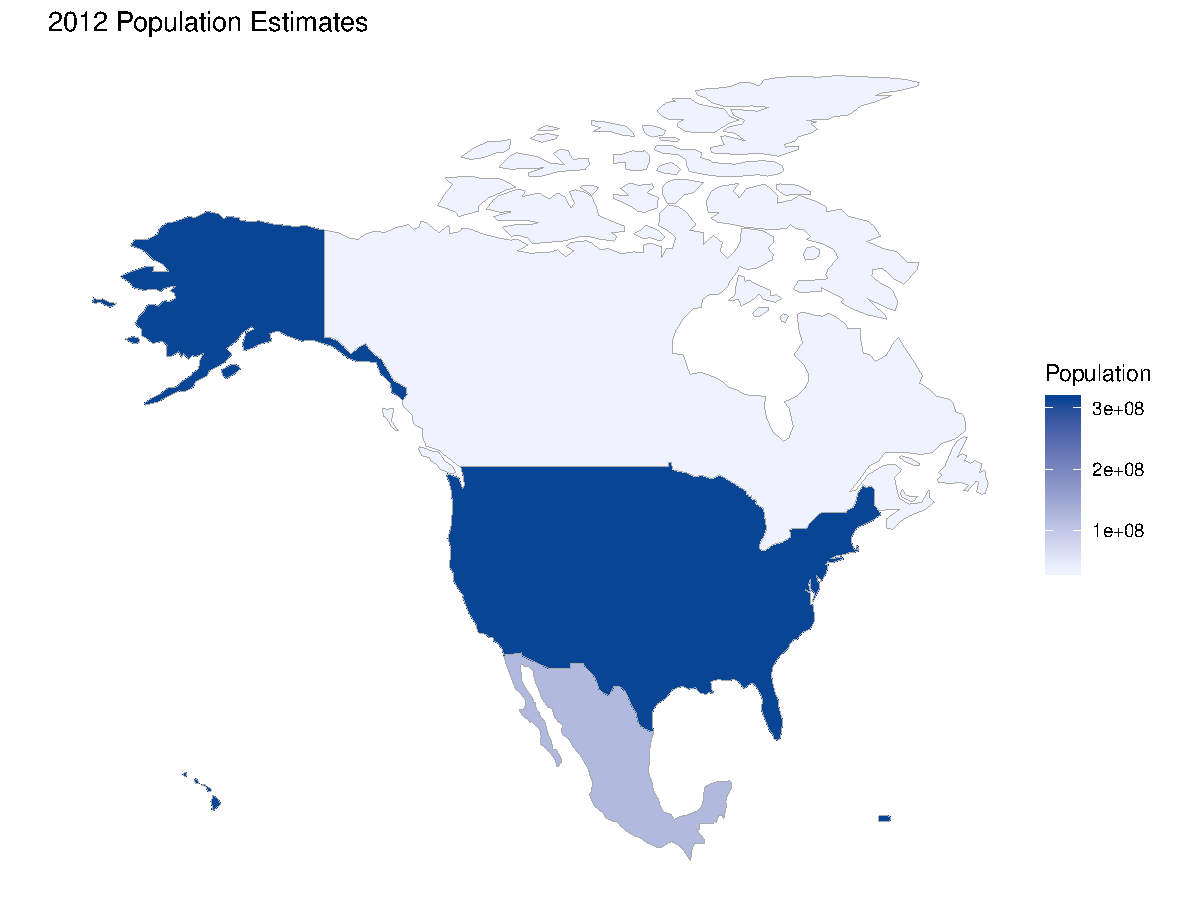
\includegraphics{Choroplethen_files/figure-beamer/unnamed-chunk-24-1.pdf}

\end{frame}

\begin{frame}[fragile]{\href{http://mirrors.softliste.de/cran/web/packages/choroplethr/vignettes/d-country-choropleth.html}{Choroplethen
Länder}}

\begin{Shaded}
\begin{Highlighting}[]
\KeywordTok{data}\NormalTok{(df_pop_country)}
\KeywordTok{country_choropleth}\NormalTok{(df_pop_country,}
              \DataTypeTok{title      =} \StringTok{"2012 Population Estimates"}\NormalTok{,}
              \DataTypeTok{legend     =} \StringTok{"Population"}\NormalTok{,}
              \DataTypeTok{num_colors =} \DecValTok{1}\NormalTok{,}
              \DataTypeTok{zoom       =} \KeywordTok{c}\NormalTok{(}\StringTok{"united states of america"}\NormalTok{,}
                             \StringTok{"mexico"}\NormalTok{, }\StringTok{"canada"}\NormalTok{))}
\end{Highlighting}
\end{Shaded}

\end{frame}

\begin{frame}{\href{http://mirrors.softliste.de/cran/web/packages/choroplethr/vignettes/d-country-choropleth.html}{Choroplethen
Länder}}

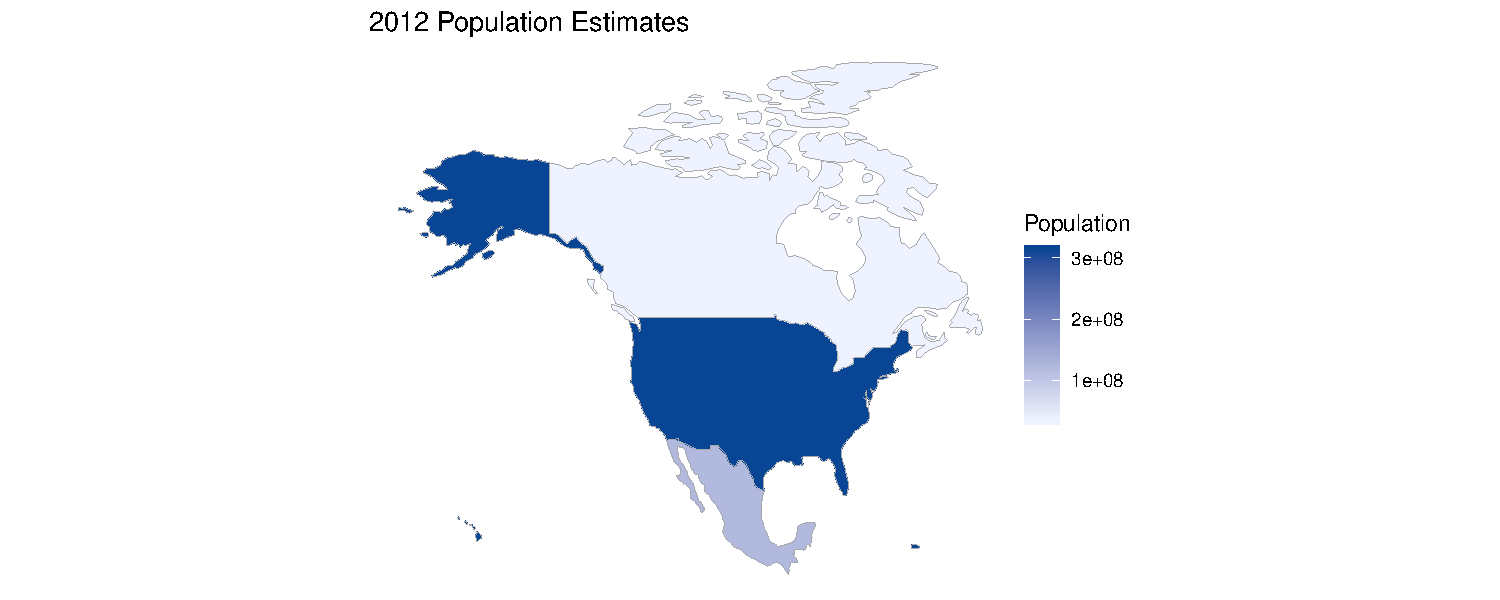
\includegraphics{Choroplethen_files/figure-beamer/unnamed-chunk-26-1.pdf}

\end{frame}

\begin{frame}[fragile]{Weltbank Daten}

\begin{Shaded}
\begin{Highlighting}[]
\KeywordTok{library}\NormalTok{(WDI) }
\KeywordTok{choroplethr_wdi}\NormalTok{(}\DataTypeTok{code=}\StringTok{"SP.POP.TOTL"}\NormalTok{, }\DataTypeTok{year=}\DecValTok{2012}\NormalTok{, }
                \DataTypeTok{title=}\StringTok{"2012 Population"}\NormalTok{, }
                \DataTypeTok{num_colors=}\DecValTok{1}\NormalTok{)}
\end{Highlighting}
\end{Shaded}

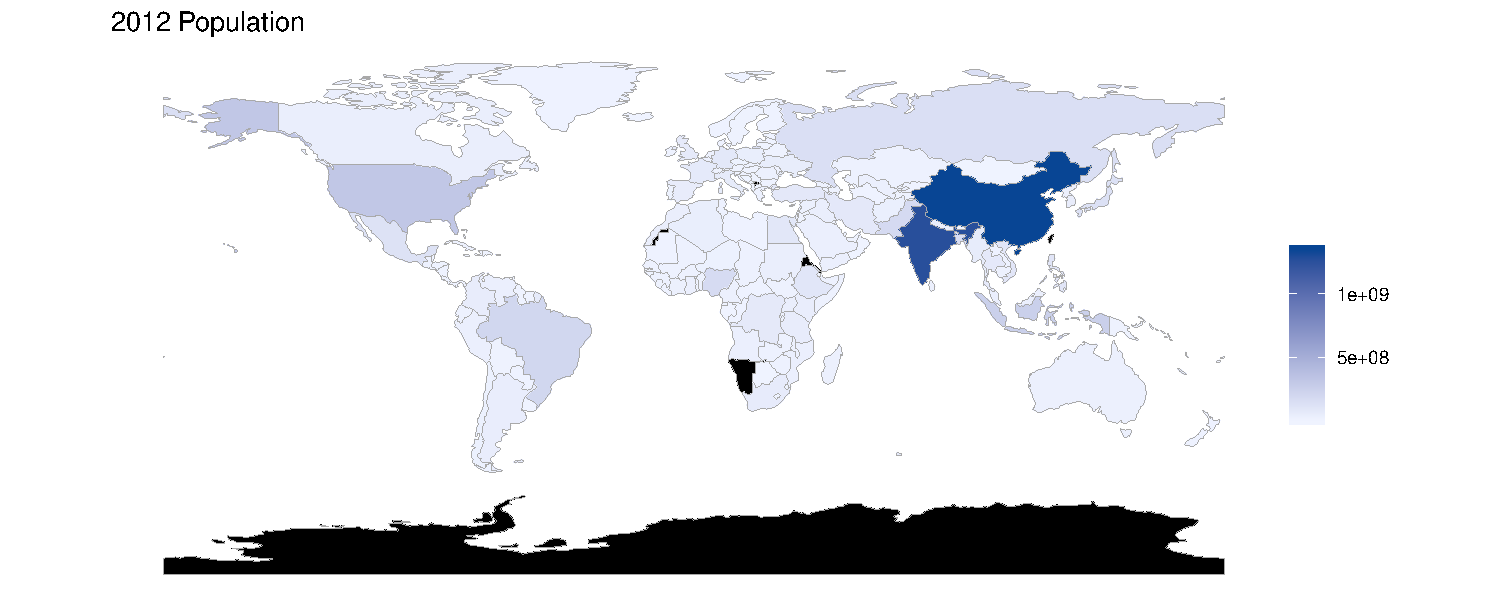
\includegraphics{Choroplethen_files/figure-beamer/unnamed-chunk-27-1.pdf}

\end{frame}

\begin{frame}[fragile]{\href{http://mirrors.softliste.de/cran/web/packages/choroplethr/vignettes/f-world-bank-data.html}{Lebenserwartung}}

\begin{Shaded}
\begin{Highlighting}[]
\KeywordTok{choroplethr_wdi}\NormalTok{(}\DataTypeTok{code=}\StringTok{"SP.DYN.LE00.IN"}\NormalTok{, }\DataTypeTok{year=}\DecValTok{2012}\NormalTok{,}
                \DataTypeTok{title=}\StringTok{"2012 Life Expectancy"}\NormalTok{)}
\end{Highlighting}
\end{Shaded}

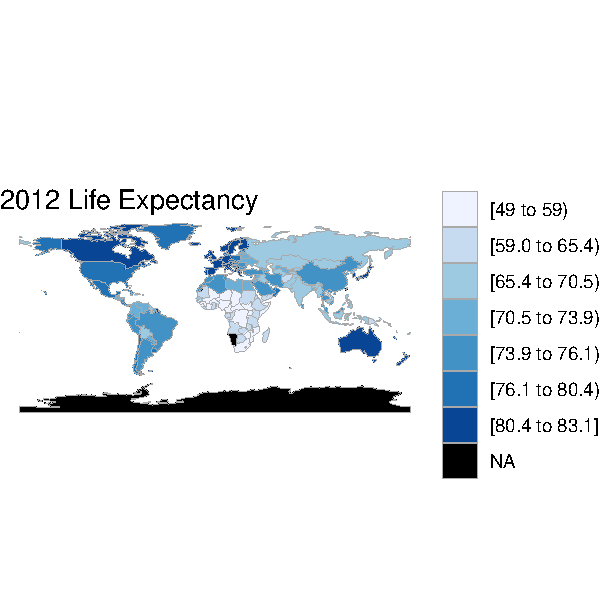
\includegraphics{Choroplethen_files/figure-beamer/unnamed-chunk-28-1.pdf}

\end{frame}

\begin{frame}[fragile]{Ein weiterer Datensatz}

\begin{quote}
A data.frame containing all US presdiential election results from 1789
to 2012
\end{quote}

\begin{Shaded}
\begin{Highlighting}[]
\KeywordTok{data}\NormalTok{(df_president_ts)}
\end{Highlighting}
\end{Shaded}

D = Democratic; R = Republican; PR = Progressive;

\begin{longtable}[]{@{}lllllllll@{}}
\toprule
& region & 1908 & 1912 & 1916 & 1920 & 1924 & 1928 & 1932\tabularnewline
\midrule
\endhead
42 & south dakota & R & PR & R & R & R & R & D\tabularnewline
43 & tennessee & D & D & D & R & D & R & D\tabularnewline
44 & texas & D & D & D & D & D & R & D\tabularnewline
45 & utah & R & R & D & R & R & R & D\tabularnewline
46 & vermont & R & R & R & R & R & R & R\tabularnewline
47 & virginia & D & D & D & D & D & R & D\tabularnewline
48 & washington & R & PR & D & R & R & R & D\tabularnewline
\bottomrule
\end{longtable}

\begin{Shaded}
\begin{Highlighting}[]
\CommentTok{# install.packages("choroplethrMaps")}
\KeywordTok{library}\NormalTok{(}\StringTok{"choroplethrMaps"}\NormalTok{)}
\end{Highlighting}
\end{Shaded}

\end{frame}

\begin{frame}[fragile]{Resourcen}

\begin{Shaded}
\begin{Highlighting}[]
\KeywordTok{citation}\NormalTok{(}\StringTok{"choroplethr"}\NormalTok{)}
\end{Highlighting}
\end{Shaded}

\begin{verbatim}
## 
## To cite package 'choroplethr' in publications use:
## 
##   Ari Lamstein (2018). choroplethr: Simplify the Creation of
##   Choropleth Maps in R. R package version 3.6.3.
##   https://CRAN.R-project.org/package=choroplethr
## 
## A BibTeX entry for LaTeX users is
## 
##   @Manual{,
##     title = {choroplethr: Simplify the Creation of Choropleth Maps in R},
##     author = {Ari Lamstein},
##     year = {2018},
##     note = {R package version 3.6.3},
##     url = {https://CRAN.R-project.org/package=choroplethr},
##   }
\end{verbatim}

\end{frame}

\begin{frame}[fragile]{Resources / Links}

\begin{itemize}
\item
  \href{https://cran.r-project.org/web/packages/choroplethr/vignettes/a-introduction.html}{\textbf{Einführung
  - Was sind Choroplethen}}
\item
  \href{http://radar.oreilly.com/2014/01/new-choropleth-package-in-r.html}{\textbf{Beschreibung}}
  der Nutzung des \texttt{choroplethr} Paketes
\item
  Die
  \href{https://cran.r-project.org/web/packages/choroplethr/vignettes/b-state-choropleth.html}{\textbf{US
  Staaten}} plotten mit \texttt{choroplethr}
\item
  \href{https://cran.r-project.org/web/packages/choroplethr/vignettes/f-world-bank-data.html}{\textbf{Weltbankdaten
  in Karten darstellen}} mit \texttt{choroplethr}
\item
  \href{http://blog.revolutionanalytics.com/2014/01/easy-data-maps-with-r-the-choroplethr-package-.html}{\textbf{Revolutions-Blog}}
  über das \texttt{choroplethr} Paket
\item
  \href{http://www.trulia.com/tech/2014/01/15/the-choroplethr-package-for-r/}{\textbf{trulia}}-blog
  über das \texttt{choroplethr} Paket
\item
  \href{http://www.r-bloggers.com/slides-for-my-upcoming-talk-mapping-census-data-in-r/}{\textbf{Präsentation
  von Ari Lamstein}} über das \texttt{choroplethr} Paket
\end{itemize}

\end{frame}

\end{document}
